\documentclass[11pt,a4paper]{article}
\usepackage[T1]{fontenc}
\usepackage{lmodern}
\usepackage[margin=27mm,headheight=15pt]{geometry}
\usepackage{amsmath,amssymb,amsthm,mathtools}
\usepackage{microtype,booktabs,longtable,tabularx,array,enumitem}
\usepackage{xcolor,graphicx,tikz,fancyhdr,listings}
\usetikzlibrary{arrows.meta,positioning}
\definecolor{Accent}{HTML}{234E70}
\definecolor{Pale}{HTML}{F2F5F8}
\usepackage[colorlinks=true,linkcolor=Accent,citecolor=Accent,urlcolor=Accent]{hyperref}
\usepackage[nameinlink,noabbrev]{cleveref}
\hypersetup{pdftitle={Few Nonlinear Columns: Fixed-Parameter Forest Selection for Compressed Unknot Hierarchies},pdfauthor={Research continuation for the ProveIt project}}
\newtheorem{theorem}{Theorem}[section]
\newtheorem{lemma}[theorem]{Lemma}
\newtheorem{proposition}[theorem]{Proposition}
\newtheorem{corollary}[theorem]{Corollary}
\theoremstyle{definition}
\newtheorem{definition}[theorem]{Definition}
\newtheorem{example}[theorem]{Example}
\newtheorem{remark}[theorem]{Remark}
\newcommand{\supp}{\operatorname{supp}}
\newcommand{\cl}{\operatorname{cl}}
\newcommand{\rank}{\operatorname{rank}}
\newcommand{\Reach}{\operatorname{Reach}}
\newcommand{\Stop}{\operatorname{Stop}}
\newcommand{\Ftwo}{\mathbb F_2}
\newcommand{\bits}{\operatorname{bits}}
\setlist{itemsep=3pt,topsep=5pt}
\setlength{\emergencystretch}{2em}
\pagestyle{fancy}
\fancyhf{}
\fancyhead[L]{\small\color{Accent}Few nonlinear columns}
\fancyhead[R]{\small ProveIt research continuation}
\fancyfoot[C]{\thepage}
\renewcommand{\headrulewidth}{0.3pt}
\lstset{basicstyle=\small\ttfamily,breaklines=true,columns=fullflexible,keepspaces=true,frame=single,rulecolor=\color{Accent!30},backgroundcolor=\color{Pale},showstringspaces=false}
\title{\color{Accent}\textbf{Few Nonlinear Columns}\\[5pt]
\Large Fixed-Parameter Forest Selection\\for Compressed Unknot Hierarchies}
\author{Research continuation prepared for\\Vladimir Reshetnikov's ProveIt project}
\date{12 October 2026}
\begin{document}
\maketitle
\begin{abstract}
We resolve a parameterized forest-selection problem explicitly left open by
the recent ProveIt research on dual-forest normalization. A candidate forest
removes top handles; the remaining unsigned occurrence matrix must admit
complete unit-column peeling. Columns supported on two rows give directed
implications and a polynomial independent-transversal problem. A column
with three unit entries introduces a two-premise activation rule.

If there are $k$ such nonlinear columns, we give an exact deterministic
algorithm with cost $3^k B_{2k+1}\operatorname{poly}(N)$, where $N$ is the
encoded input length and $B_j$ is a Bell number. The exponential factor
depends on the nonlinear columns, while the number of top handles may be
arbitrary. An initial event-order proof isolates at most $2k$ residual demands.
A sharper reduction dispenses with event-order enumeration: one
distinguished partition block records undemanded prerequisites, while
other blocks share forest witnesses before matroid intersection. We also prove a weighted
optimization extension and a sharper rank-layer reduction for columns
satisfying the native boundary-of-boundary identity.

The accompanying exact Python implementation constructs independently
checkable positive and negative certificates. Fresh source reconstruction,
independent finite oracles, controlled performance comparisons, and detailed
integration contracts distinguish the proved finite operator from its
topological use. The result is a local algorithmic advance toward compressed
hierarchies. A bound on the nonlinear parameter along every unknot hierarchy,
efficient surface discovery, and global control of hierarchy visits remain
separate mathematical obligations.
\end{abstract}
\clearpage
\tableofcontents
\newpage
\section{Problem, contribution, and relation to the current repository}
\label{sec:position}

The computational target is an exact recognizer with a proved
quasi-polynomial worst-case bound in the original diagram size. The present
contribution addresses one definite obstruction inside that programme:
\emph{choose a legal top-handle forest so that the surviving raw attaching
relations can all be eliminated}. For a fixed forest, this is already a
linear-work peeling problem. Finding a good forest is the difficult part.

The newest dual-forest-normalization package proves a polynomial algorithm
when every column containing a unit entry meets at most two rows. It asks
explicitly for a parameterized extension to the remaining native column
shape $(1,1,1)$ \cite{repo-dual-normalization}. We supply that extension.
The resulting theorem applies to arbitrary supplied finite occurrence
systems with the stated shape; geometric authentication is required only
when interpreting a successful matrix certificate as handle cancellation.

\subsection{Exact source boundary}

The inspected repository head was
\begin{center}
\small\texttt{ada929648530f8689c26426e132a1b3e1c69c724}.
\end{center}
Its maintained \texttt{fast/} subtree has Git object identity
\begin{center}
\small\texttt{697afe0edf113951dd53f8fe9b4c5011f6227b94}.
\end{center}
All 913 files in that subtree were checked byte-for-byte against their
Git blob identities. The local baseline is the preceding commit
\texttt{c6d0ec8aa0b6308310ab6c081ba29d8bc363ede5}; the inspected head adds
the relative-top-handles archive and does not alter the maintained runtime.
All six archives then present in \texttt{docs/incoming/} were extracted and
matched to their published Git blob hashes before their contents were used.
The provenance files in this package retain those identities.

The incoming work is substantial. It would be incorrect to describe its
forest, stopping-set, and compression results as new results of this paper.
The following table states the relevant difference in scope.

\begin{center}
\small
\begin{tabularx}{\linewidth}{@{}p{.29\linewidth}X@{}}
\toprule
Earlier contribution & Relation to the present result \\
\midrule
Dual-forest normalization & Polynomial two-row-column case; general
obstruction-guided search parameterized by top-forest depth. We allow
nonlinear columns with fixed-parameter dependence on their number. \\
Relative top handles & Source-relative elimination and a kernel for
exceptional \emph{rows} after a fixed forest. Our parameter counts
\emph{columns}, and the forest is selected during the algorithm. \\
Positive cancellation & Exact completion by immutable column peeling,
deferral, and passive-count transport. We use its completion criterion. \\
Dual forests and homological progress & Native weighted forest heuristics
and an algebraic progress certificate. Our weighted theorem optimizes over
\emph{successful} forests under the nonlinear parameter bound. \\
Component-gauge cut atlases & Exact small-cut queries on supplied graph
grammars; a different graph operation from selecting handle-cancellation
forests. \\
Flag regularization & Compressed regular cell structures and a controlled
Morse interface; it does not perform the forest search solved here. \\
\bottomrule
\end{tabularx}
\end{center}

\subsection{Current external mathematical baseline}

Lackenby's February 2021 Davis slides announce $n^{O(\log n)}$, while his
March 2021 Oxford slides state $2^{O((\log n)^3)}$ and explain the latter
using a hierarchy length of order $(\log n)^2$ and a polynomial pattern
bound \cite{lackenby-davis,lackenby-oxford}. These are two dated formulations
of the announced programme and should not be silently identified.

The July 2026 preprint gives a rigorous hierarchy framework. Proposition
9.1 bounds step visits in terms of hierarchy length and pattern complexity;
Theorem 14.4 supplies polynomial encoded-time cutting and parallelity-bundle
information. The manuscript leaves further acceleration to future work
\cite{lackenby2026}. Our local selection theorem fits between the
compressed geometric construction and its subsequent cancellation test.

\subsection{Attribution and novelty boundary}

Sets generating every variable under definite-Horn closure are usually
called \emph{keys}. Symmetric all-but-one implications are studied as
hypergraph Horn functions \cite{horn-keys,hypergraph-horn}. Column peeling
also has established connections to stopping sets and triangular matching
patterns \cite{stopping-sets,uniquely-restricted}. Independent transversals
and their algorithmic solution are classical matroid theory
\cite{rado,edmonds}.

The contribution here is the bounded-event reduction with an external
forest constraint: mandatory unary source components absorb all but a
bounded family of predecessor requirements; the remaining requirements can
share witnesses and are handled by a set-partition reduction. A separate
geometric rank invariant sharpens this reduction on authenticated native
incidence data. We did not identify this exact parameterized theorem in a
focused primary-source search. That search and the repository audit support
the stated project contribution; they do not establish worldwide priority.

The mathematical arguments are research-draft proofs, backed by independent
computational checks. They have not been formalized in a proof assistant or
subjected to journal peer review. The package contains all details needed
to scrutinize the claims at the finite-operator level.

\section{Unsigned cancellation and its geometric input}
\label{sec:model}

\subsection{The finite decision problem}

Let $R$ be a finite set of row labels and $C$ a finite set of columns. The
matrix $A=(a_{rc})$ has nonnegative integer entries and is stored sparsely.
Each row either labels one edge of a finite connected undirected
multigraph $G$ or is declared unavailable for top cancellation. The graph
has a distinguished exterior vertex $0$. Parallel edges are distinct row
labels; loops cannot belong to a forest. Write $E\subseteq R$ for the
eligible nonloop edges and $r=|V(G)|-1$ for the rank.

A top choice is a spanning tree $T\subseteq E$. It removes the rows of
$T$. On the remaining row set $L$, a column $c$ is a legal leaf when
\[
                         \sum_{r\in L}a_{rc}=1.
\]
There is then a unique row $u\in L$ with $a_{uc}=1$; delete $u$ and
record the pair $(u,c)$. Continue until every row is deleted or no leaf
remains. The input question is whether \emph{some} top tree gives complete
peeling. Rows unavailable for top cancellation can still be deleted by
leaf pivots; excluding them from the matrix would change the problem.

\begin{lemma}[Saturation preserves the finite problem]
\label{lem:saturation}
Replacing every positive entry $a$ by $\min(2,a)$ preserves the legal
leaf predicate on every subset of rows, and therefore preserves every
peeling trace and the answer for every top tree.
\end{lemma}
\begin{proof}
A sum of nonnegative integers is one exactly when one summand is one and
every other summand is zero. Saturation preserves zero, one, and the
property of being at least two. This applies to each column on every
row subset.
\end{proof}

This observation does \emph{not} license saturating counts before a
parity or signed-chain calculation: an odd count of three would become
even. The implementation's input digest binds the uncapped integers,
and its cycle-compatibility check uses their actual parities.

\begin{definition}[Stopping set]
A nonempty subset $S\subseteq R$ is a stopping set if every column sum
$\sum_{r\in S}a_{rc}$ is zero or at least two.
\end{definition}

\begin{proposition}[Exact immutable obstruction]
\label{prop:stopping}
Peeling a row subset $L$ completes if and only if $L$ contains no stopping
set. Its final residue is independent of the order of legal leaf choices
and equals the union of all stopping subsets of $L$.
\end{proposition}
\begin{proof}
A stopping set cannot lose its first row to a legal leaf: the corresponding
column would already have sum at least two inside that stopping set.
Consequently every stopping subset remains throughout every peeling
execution. Conversely, a nonempty terminal residue has no unit column and
is itself stopping. The union of stopping sets is stopping: for a column
with a positive contribution to the union, one constituent stopping set
already contributes at least two. The union of all stopping subsets is therefore the largest stopping
residue, possibly empty. Every terminal residue contains this union, and a
nonempty terminal residue is itself stopping and hence contained in it.
If the union is empty, all executions complete.
\end{proof}

The preceding incoming reports prove that complete positive raw
cancellation can always be witnessed by such immutable column peeling
\cite{repo-positive,repo-dual-normalization}. This completion theorem is
the reason a search over more complicated positive substitutions is
unnecessary for the present decision problem. A certificate below uses
only the original matrix entries and an ordinary tree.

\subsection{Activation reverses the viewpoint}

Call a removed row \emph{active}. A top tree is the initial active set.
A column with support $H$ can activate its row $u$ exactly when
\[
               a_{uc}=1,\qquad H\setminus\{u\}\subseteq X,
\]
where $X$ is the current active set. Thus it gives the Horn rule
$H\setminus\{u\}\to u$ for each of its unit entries. A column with no
unit entry gives no rule. A unit singleton is an unconditional rule;
two-row supports give directed unary rules. Supports of three or more
rows are the nonlinear part of the system.

The closure $\cl_A(X)$ is obtained by repeatedly applying all legal
rules. Finite monotonicity shows that it exists and is independent of the
application order. The tree $T$ is successful exactly when
$\cl_A(T)=R$. This is an independent-key problem for a Horn closure,
where independence is taken in an external graphic matroid.

\subsection{Source-relative geometric interpretation}

The native complementary core is a handle structure obtained from an
authenticated triangulation and normal coordinate vector. After fixing
the lower $0/1$ forest, its surviving one-handle cocores index columns.
Two-handle attaching curves give \emph{geometric occurrence counts};
algebraic exponent sums cannot replace them. The cap graph records the
two actual three-handle ends of each source two-handle, with exposed ends
sent to the exterior root. Its rooted spanning trees give legal $2/3$
cancellation schedules under the source-relative theorem proved in the
incoming packages \cite{repo-dual-normalization,repo-relative-top}.

After top cancellation, an immutable column leaf supplies a one/two
cancellation in the already authenticated source model. Finite bundle
boundary relations must also be included. In particular, later annular
rows are not eligible cap edges and are represented as unavailable rows.
Their omission would turn an incomplete core criterion into an unsound
whole-cut criterion.

The graph--matrix algorithm does not independently certify that these
data arise from a manifold. Its positive output becomes a geometric
certificate only after the cap graph, the occurrence matrix, and the
required relative charts have been reconstructed and checked. A negative
output says that this \emph{fixed raw forest-and-peeling criterion} cannot
complete. It does not say that the cut piece is not a handlebody, or that
the original knot is nontrivial.

\subsection{Why the exceptional column shape is natural}

For original native one-handle cocores, a triangular source-face region
has at most three actual boundary occurrences. A column containing a
unit and more than two owners therefore has precisely three distinct
unit owners. Moreover, the raw parity incidences obey the
boundary-of-boundary identity \cite{repo-dual-normalization}. The new
source audit rechecks these properties before saturation. It also finds
the same three-occurrence bound on every reconstructed finite boundary
matrix in the maintained corpus. The latter is an experimental statement
about those matrices, not a universal theorem about arbitrary interfaces.

The parameter $k$ will count nonlinear columns after free cancellations.
The local theorem supplies no uniform polylogarithmic bound on $k$ in
the original crossing number, and does not derive one from the underlying
manifold type or from the number of bits per normal coordinate. Establishing useful
geometric control of $k$ is one of the main next questions.

% Section fragment for the parent article; requires amsmath, amssymb,
% amsthm, and theorem/lemma/proposition/corollary environments.
\section{Few nonlinear columns: an exact fixed-parameter forest algorithm}
\label{sec:fpt-column-theorem}

Let $R$ be the row set of the immutable nonnegative occurrence matrix,
and let $E\subseteq R$ label all nonloop edges of a connected undirected
multigraph $G$. Parallel edges are allowed; other rows are matroid loops. A selected forest
activates its rows initially. A unit-column pivot activates its last
remaining row. We use the established equivalence between complete
positive raw cancellation and complete unit-column peeling for this
fixed source presentation.

An active column has at least one entry equal to one; a column without
such an entry is inert for unit peeling. Form the ordinary implication
digraph $P$ on $R$ from all active columns supported on at most two rows.
A singleton unit column contributes its row to the seed set $Z$.
A two-row column supported on $u,v$ contributes $v\to u$ if its entry
at $u$ is one, and $u\to v$ if its entry at $v$ is one. Thus a
$(1,1)$ column contributes both directions and a $(1,a)$ column with
$a\ge2$ contributes only the direction towards the unit entry.

Let $H_1,\ldots,H_k$ be the supports of the remaining active columns.
Assume each consists of three distinct unit owners. Each such column
contributes the three implications
\[
                  H_i\setminus\{x\}\longrightarrow x
                  \qquad(x\in H_i).
\]
Ordinary implication closure is directed reachability in $P$, denoted
$\operatorname{Reach}_P$. The full activation closure additionally uses
these two-premise implications. An exceptional column can produce at
most one newly activated row: after its first useful application, all
three of its support rows are active.

\subsection{Removing the closure that is free for every tree}

Write $\cl_A(X)$ for the rows activated by unit peeling
from an initial row set $X$, including all singleton-unit seeds. Compute
the \emph{free closure}
\[
                         W=\cl_A(\varnothing).
\]
This preprocessing involves no choice of top forest. Restrict the
matrix columns to the live rows $R_0=R\setminus W$, keeping their
coefficients unchanged.

\begin{proposition}[Exact free-closure preprocessing]
\label{prop:fpt-free-closure}
For every initially selected row set $X\subseteq R$,
\[
 \cl_A(X)
   =W\cup
     \cl_{A[R_0]}(X\setminus W).
\]
Consequently the exceptional-column parameter may be measured after
this preprocessing. The original cap graph and every original eligible
edge must remain available for tree completion and weight optimization.
\end{proposition}
\begin{proof}
The activation rule for a unit entry in row $x$ requires all other
support rows of its column to have been activated. Every row of $W$ is
active from every initial set $X$, by monotonicity. Once these rows are
active, the rules with outputs in $R_0$ have precisely the prerequisites
obtained by restricting their columns to $R_0$. Each residual activation
is therefore valid in the original system after activating $W$.
Conversely, remove from an original activation schedule the events whose
outputs lie in $W$. Every remaining event has all of its remaining
prerequisites activated earlier in the residual schedule, giving the
reverse inclusion. A column used during free peeling has no live owner
afterwards, so it cannot create a conflict through reuse.
\end{proof}

One convenient implementation retains all original row labels, marks
the rows of $W$ as free seeds, and removes them only from the residual
column supports. Their vertices then have no residual clauses. This
keeps the original connected graph and its eligible edge set unchanged.
Equivalently, discarded free rows may be retained as extension-only graph
edges. A column losing one of its three unit owners becomes an ordinary
two-row column, so the residual value of $k$ cannot increase. Authenticate
any geometric parity identity from the uncapped source counts before
capping multiplicities.

Henceforth, recompute $P,H_1,\ldots,H_k$ from the residual columns,
retain the original $R,E,G$, and include every row of $W$ in $Z$.
The rows of $W$ are isolated free seeds in the residual implication
system. All subsequent parameters refer to this recomputed system.

\begin{theorem}[Fixed-parameter forest selection by exceptional columns]
\label{thm:column-fpt}
The existence of a spanning tree $T\subseteq E$ whose complementary
rows peel completely can be decided deterministically in
\[
       3^k k! B_{2k}\,\operatorname{poly}(N)
       =2^{O(k\log(k+2))}\operatorname{poly}(N)
\]
bit operations, where $N$ is the encoded graph--matrix input length and
$B_j$ is the $j$th Bell number. A successful tree and an immutable-source
peeling schedule can be constructed within this bound. The algorithm
enumerates no $|R|^k$ family of forest-edge choices.
\end{theorem}

The parameter in this theorem is the number of exceptional
\emph{columns}, and the algorithm chooses the forest jointly with the
peeling strategy. It is therefore distinct from an algorithm that fixes
the forest first or parameterizes exceptional rows. Its proof follows
from a reduction to classical independent transversals; no matroid
property is assumed for the family of peelable row sets.

\subsection{Ordered exceptional events}

A \emph{scenario} consists of a permutation $i_1,\ldots,i_k$ of the
exceptional columns and an output choice $o_j\in H_{i_j}$ for each
position. At event $j$, the two rows of $H_{i_j}\setminus\{o_j\}$
must already be active, and $o_j$ becomes active. An output already
active is allowed; the event then has no effect. There are $3^k k!$
scenarios, including one empty scenario when $k=0$.

\begin{lemma}[Complete scenario family]
\label{lem:fpt-scenarios-complete}
Every successful forest admits a complete activation schedule obeying
one of these scenarios. Conversely, a legal scenario execution that
activates every row certifies success of its initial forest.
\end{lemma}
\begin{proof}
Take a complete activation schedule and list, in their actual order,
the exceptional-column applications that activate a new row. No column
appears twice in this list. Append every unused exceptional column after
the original schedule finishes, choosing its output arbitrarily. These
appended events are legal because all rows are already active. The
converse follows directly from the implication rules: each useful
exceptional event is a column with exactly one unit occurrence remaining.
Ordinary directed reachability is implemented by the corresponding
two-row or singleton unit columns.
\end{proof}

Fix a scenario and write $O=\{o_1,\ldots,o_k\}$. Let
$Q_1,\ldots,Q_p$ be those source strongly connected components of $P$
that meet neither $Z$ nor $O$, and put
\[
              A_\ell=Q_\ell\cap E,\qquad
              U=Z\cup\bigcup_{\ell=1}^p Q_\ell.
\]
The sets $A_\ell$ are pairwise disjoint. Every complete execution of
this scenario must select a row in each $A_\ell$: no ordinary arc enters
$Q_\ell$, and no chosen exceptional event outputs into it. Conversely,
one selected row in $Q_\ell$ activates all of $Q_\ell$ by strong
connectivity. These are obligations \emph{conditioned on the scenario};
they need not be stopping sets of the full matrix when exceptional
columns are present.

For a prerequisite $x\in H_{i_j}\setminus\{o_j\}$ at event $j$, set
\[
 C_j=\operatorname{Reach}_P
         \bigl(U\cup\{o_1,\ldots,o_{j-1}\}\bigr).
\]
If $x\in C_j$, no additional requirement is needed. Otherwise introduce
the \emph{predecessor demand}
\[
 D_{j,x}=\{e\in E:
              x\in\operatorname{Reach}_P(\{e\})\}.
 \tag{$\ast$}\label{eq:fpt-predecessor-demand}
\]
There are at most $2k$ retained demands. Repeated demands may be kept as
separately indexed requirements. Only earlier outputs occur in $C_j$;
using future outputs would permit circular activation justifications.

\begin{lemma}[Separation of the residual demands]
\label{lem:fpt-demand-separation}
Every retained predecessor demand is disjoint from every $A_\ell$.
\end{lemma}
\begin{proof}
If $e\in A_\ell\cap D_{j,x}$, then $e\in Q_\ell\subseteq U$ and
there is a directed path from $e$ to $x$. Consequently $x\in C_j$, in
contradiction to retention of this demand.
\end{proof}

\begin{proposition}[Exact requirements for a fixed scenario]
\label{prop:fpt-fixed-scenario}
An independent edge set $F$ supports complete activation according to the
fixed scenario if and only if $F$ meets every $A_\ell$ and every retained
predecessor demand.
\end{proposition}
\begin{proof}
For necessity, the source-component argument gives the requirements
$F\cap A_\ell\ne\varnothing$. Immediately before event $j$, every
active row belongs to
\[
 \operatorname{Reach}_P
       \bigl(Z\cup F\cup\{o_1,\ldots,o_{j-1}\}\bigr).
\]
A prerequisite $x\notin C_j$ is not reached from $Z$ or an earlier
output. Reachability from a union is the union of the individual
reachability sets, so some $e\in F$ reaches $x$. This is precisely a
witness in $F\cap D_{j,x}$.

For sufficiency, meeting $A_\ell$ activates every vertex of $Q_\ell$;
hence all of $U$ is available. Induct on the prescribed events. A
prerequisite in $C_j$ is reached from already justified sources or earlier
outputs. Every other prerequisite is reached from a selected edge in its
demand. Thus event $j$ is legal. After the final event every source
component of $P$ contains a singleton seed, a selected edge, or a chosen
output. Every component of a finite acyclic condensation is reachable
from a source component, so ordinary reachability activates every row.
\end{proof}

\subsection{Partitioning the few demands}

The retained demands can overlap and can share a single selected edge.
Requiring a different selected edge for each would be incorrect. The
following elementary lemma isolates the finite combinatorics needed to
handle shared witnesses.

\begin{lemma}[Partition reduction for an independent hitting set]
\label{lem:fpt-partition-reduction}
Let $M$ be a finite matroid on $E$. Let $A_1,\ldots,A_p$ be pairwise
disjoint subsets of $E$, and let $D_1,\ldots,D_q$ be subsets of
$E\setminus\bigcup_\ell A_\ell$. There is an $M$-independent set
meeting every $A_\ell$ and every $D_j$ if and only if, for some set
partition $\pi$ of $\{1,\ldots,q\}$, the family
\[
       A_1,\ldots,A_p,\qquad
       K_B=\bigcap_{j\in B}D_j\quad(B\in\pi)
\]
has an independent system of distinct representatives.
\end{lemma}
\begin{proof}
Given an independent hitting set $F$, choose $e_j\in F\cap D_j$ and
partition the demand indices according to equality of their chosen
witnesses. For every block $B$, its common witness belongs to $K_B$;
witnesses for different blocks are distinct. Also choose a representative
in $F\cap A_\ell$ for each $\ell$. The latter representatives are
pairwise distinct because the $A_\ell$ are disjoint, and none equals a
demand witness because each $D_j$ avoids their union. All representatives
form a subset of the independent set $F$. Conversely, representatives
for the displayed groups meet all original demands and mandatory groups.
The empty demand family uses the unique empty set partition.
\end{proof}

For each partition, solve the independent-transversal problem in the
graphic matroid of $G$. Its groups may overlap. To reduce to the familiar
graphic/partition intersection, give every membership $e\in K$ its own
edge copy $(K,e)$, with the same graph endpoints as $e$. Use the graphic
matroid on these copies and the partition matroid allowing at most one
edge in each required group. Two copies of the same original nonloop
edge are parallel and hence dependent; copies of an original loop remain
loops. A common independent set of size equal to the number of groups
therefore projects to an independent system of distinct original-edge
representatives. There are at most $(q+1)|E|$ copies, not $|E|^q$.

Rado's independent-transversal theorem gives the exact alternative:
either these groups have independent representatives or some subfamily
$\mathcal J$ satisfies
\[
 \rho_G\left(\bigcup_{K\in\mathcal J}K\right)<|\mathcal J|.
 \tag{$\dagger$}\label{eq:fpt-rado-obstruction}
\]
Here the union is a set of original edge labels. Repeated membership does
not increase rank. This is a classical matroid result; the present
reduction supplies the scenario-specific groups to which it applies.

\begin{proof}[Proof of Theorem~\ref{thm:column-fpt}]
Enumerate all scenarios. For each, compute its source groups and at most
$2k$ retained demands. Enumerate their set partitions and solve each
graphic/partition intersection problem. By
Lemma~\ref{lem:fpt-demand-separation},
Lemma~\ref{lem:fpt-partition-reduction} applies; by
Proposition~\ref{prop:fpt-fixed-scenario}, a successful intersection
produces a successful forest. Extend it to a spanning tree. Activation
is monotone in the initially selected rows, so this extension remains
successful; replay peeling directly against the immutable source matrix.

Conversely, any successful tree admits a scenario by
Lemma~\ref{lem:fpt-scenarios-complete}. For that scenario it meets all
required groups and demands. The partition reduction therefore makes
at least one of its matroid-intersection subproblems successful.

There are $3^k k!$ scenarios and at most $B_{2k}$ partitions for each.
All residual constructions and matroid computations are polynomial in
the encoded input size. For $k\ge1$,
\[
      3^k k!B_{2k}
      \le3^k k^k(2k)^{2k}=(12k^3)^k,
\]
which proves the stated bound. Scenarios and partitions can be streamed,
so the producer needs only polynomial working space apart from any
explicitly retained negative certificate.
\end{proof}

\subsection{Independent positive and negative certificates}

A positive certificate consists simply of the selected tree and the
complete peeling schedule. Its checker need not trust, or reproduce,
the scenario search or the matroid-intersection implementation.

For a negative certificate, record a violated inequality
\eqref{eq:fpt-rado-obstruction} for every scenario/partition subproblem.
An independent verifier regenerates the canonical enumeration, derives
each family of requirements, checks that every subproblem is covered,
and verifies the reported rank defect. Graphic rank is the number of
vertices minus the number of connected components of the indicated
spanning subgraph, including isolated vertices. Thus verification uses
only elementary graph operations and the explicit scenario rules; it
does not invoke matroid-intersection optimization. The resulting
certificate is fixed-parameter sized, with the same exponential
parameter factor. It is not asserted to have polynomial size for
unbounded $k$.

All conclusions concern the supplied immutable graph--matrix
certificate class. A negative result does not prove nontriviality of
the knot or exclude other handle systems, slides, subdivisions, or
hierarchy certificates.

\subsection{Optimizing the successful spanning tree}

\begin{theorem}[Minimum-weight successful tree]
\label{thm:fpt-minimum-weight-tree}
Give every eligible edge a binary-encoded signed weight. An exact
minimum-weight successful spanning tree, or proof that none exists,
can be found with the same
$2^{O(k\log(k+2))}\operatorname{poly}(N)$ parameter bound, where $N$
also includes the weight encoding length.
\end{theorem}
\begin{proof}
Fix a scenario and a demand partition, and let $L$ be the number of
required groups. Put $r=|V(G)|-1$. If $L>r$, this subproblem is
infeasible. Otherwise create its required-group copies as above and one
additional dummy copy of each original edge. The first matroid is the
graphic matroid on all copies. The second is a partition matroid with
capacity one for each required group and capacity $r-L$ for the dummy
group. Give every copy the weight of its original edge.

A common independent set of cardinality $r$ saturates every required
group and the dummy capacity. Its projection is a spanning tree
satisfying the group requirements, with exactly the same total weight.
Conversely, a spanning tree having distinct representatives for the
required groups lifts to such a common independent set: mark the
representatives by their group labels and give every remaining tree edge
its dummy label. Weighted matroid intersection therefore gives the exact
minimum tree weight for this subproblem. Minimizing over all scenarios
and partitions gives the global optimum by the completeness proof above.
Signed weights are harmless because the requested cardinality is fixed.
\end{proof}

This weighted theorem is separate from any unweighted reference
implementation. For example, negated row-occurrence counts optimize the
number of occurrences removed initially among successful trees. Such a
weight is a practical surrogate; it does not prove optimality for actual
end-to-end recognition time.

\subsection{Larger exceptional supports and quantitative regimes}

The same proof applies to an exceptional active column with support
$S_i$, size $s_i\ge3$, and nonempty set $U_i\subseteq S_i$ of
unit-coefficient owners. Its output must lie in $U_i$ and its
prerequisites are all other support rows. Put
\[
                         Q=\sum_{i=1}^k(s_i-1).
\]
There are $k!\prod_i|U_i|$ scenarios and at most $Q$ residual demands,
giving the following extension.

\begin{corollary}[Parameterization by nonlinear support]
\label{cor:fpt-nonlinear-support}
Joint forest selection and complete unit peeling with arbitrary
exceptional active columns is decidable in
\[
       k!\left(\prod_i|U_i|\right)B_Q\operatorname{poly}(N)
       =2^{O(Q\log(Q+2))}\operatorname{poly}(N).
\]
The statement remains valid for any matroid with polynomial-time
independence testing in place of the graphic matroid.
\end{corollary}
\begin{proof}
Each exceptional column still has at most one useful activation. Its
scenario event has $s_i-1$ prerequisites, so the preceding arguments
apply verbatim. Since $|U_i|\le s_i$ and $k\le Q$, the displayed
enumeration factor is $2^{O(Q\log(Q+2))}$. Cloning is a parallel
extension of the supplied matroid, and classical matroid intersection
requires only its independence oracle.
\end{proof}

For the triple-unit theorem, $k=O(\log N/\log\log N)$ gives polynomial
time, and $k=O(\log N)$ gives $N^{O(\log\log N)}$. More generally,
\[
                k\log(k+2)=O((\log N)^2)
\]
is sufficient for the quasipolynomial bound $N^{O(\log N)}$; for example,
$k=O((\log N)^2/\log\log N)$ suffices. These implications are
conditional on the corresponding parameter bound. The finite
graph--matrix theorem alone supplies no such uniform bound for all
knot diagrams.

\subsection{Authenticated cap parity preserves rank}

The general algorithm above requires no compatibility between the
occurrence matrix and the graph. The native cap incidence supplies an
additional structure when it has been independently authenticated.
Extend the graphic matroid from $E$ to the whole row set $R$ by making
rows outside $E$ matroid loops. Assume that, for every column of the \emph{full matrix used by activation},
the eligible edges with odd \emph{uncapped} occurrence count form an
even-degree subgraph of the cap graph. This includes every added
finite-boundary or interface column. The distinguished exterior vertex
is included in this condition, and a graph loop contributes degree two.

\begin{theorem}[Rank preservation of positive activation]
\label{thm:fpt-parity-rank}
Under this raw parity hypothesis, every legal unit-target activation
adds a row in the graphic-matroid closure of its prerequisite rows.
For every initial row set $X$,
\[
  \operatorname{cl}_{G}\bigl(\cl_A(X)\bigr)
                 =\operatorname{cl}_{G}(X),
  \qquad
  \rho_G\bigl(\cl_A(X)\bigr)=\rho_G(X).
\]
In particular:
\begin{enumerate}
\item every freely activated row is a graphic-matroid loop;
\item every successful independent seed is already a cap-graph basis;
\item a scenario/partition can have independent representatives only
      when its number $L$ of required groups equals
      $r=\rho_G(E)$.
\end{enumerate}
\end{theorem}
\begin{proof}
Suppose a column activates its unit row $e$. All its other support rows
are already active. If $e$ is a matroid loop, the claim is immediate.
Otherwise $e$ is a nonloop graph edge and, because its coefficient is
one, belongs to the column's odd-occurrence edge set. Every nonloop edge
in an even-degree finite multigraph lies on a cycle: if it were a bridge,
the sum of vertex degrees on one side of that bridge would be odd.
Removing $e$ from such a cycle leaves a path between its endpoints using
other odd-occurrence edges of the same column. These are among the
already active prerequisites. Hence $e$ belongs to their graphic span.
Induction over activations proves equality of the initial and final
graphic spans.

Taking $X=\varnothing$ proves the first consequence. Complete activation
has rank $\rho_G(R)=\rho_G(E)=r$; if $X$ is independent it must therefore have
cardinality $r$, proving the second. For the third, an independent
representative system is a successful independent seed by
Proposition~\ref{prop:fpt-fixed-scenario} and
Lemma~\ref{lem:fpt-partition-reduction}. Its cardinality is exactly the
number of its required groups, so $L=r$.
\end{proof}

The free-closure restriction in
Proposition~\ref{prop:fpt-free-closure} removes only matroid loops under
this authenticated hypothesis, and consequently preserves the raw
even-degree identity. By contrast, replacing an odd multiplicity at
least three by two can change parity. The rank argument must therefore
refer to the original raw counts, although the zero/unit/multiple
predicates used by the decision algorithm can still be capped at two.

\begin{corollary}[One Stirling layer suffices on parity-compatible inputs]
\label{cor:fpt-stirling-layer}
For a fixed scenario with $p$ mandatory source groups and $q$ retained
demands, the parity-compatible algorithm needs only partitions with
\[
                            |\pi|=r-p.
\]
Thus it examines $\left\{\begin{smallmatrix}q\\r-p\end{smallmatrix}\right\}$
partitions, the corresponding Stirling number of the second kind,
instead of all $B_q$ partitions. A scenario with $p>r$ or $p+q<r$
can be rejected immediately. A successful set of representatives is
already a spanning tree when the cap graph is connected.
\end{corollary}
\begin{proof}
There are $L=p+|\pi|$ required groups. The previous theorem forces
$L=r$ in every feasible subproblem. Conversely, excluding the other
partitions loses no solution: a successful tree generates, through the
partition-reduction proof, an independent representative system; rank
preservation forces that system to contain all $r$ of its tree edges.
The usual conventions include one partition of the empty set into zero
blocks and no partition into an invalid number of blocks.
\end{proof}

For a triple-unit column, the earlier source-parity audit's local
classification follows from the same hypothesis \cite{repo-dual-normalization}. Its three row elements form either a triangle of eligible edges, a
parallel pair together with a matroid loop, or three matroid loops, of
graphic ranks two, one, and zero respectively. Indeed, one nonloop edge is incompatible
with even degrees, two nonloop edges must be parallel, and three
nonloop edges must form a triangle. Only the triangle case can obtain
two prerequisites directly from a forest without another activation
route. This classification and rank pruning apply exactly where the
raw chain identity has been verified; they are not inferred merely from
an arbitrary capped matrix.

\section{Eliminating the activation-order search}
\label{sec:factorial-free}

The ordered algorithm makes causality explicit, but enumerating all $k!$
orders is unnecessary. A single distinguished block can encode the
prerequisites for which no initial-seed witness is requested. Forward
chaining then determines whether the chosen outputs can justify the other
activations. This yields the strongest bound proved in this article.

\begin{theorem}[Output choices and one distinguished partition block]
\label{thm:factorial-free}
The triple-unit forest problem is decidable, with a successful tree and
peeling certificate when one exists, in
\[
                 3^k B_{2k+1}\operatorname{poly}(N)
                 =2^{O(k\log(k+2))}\operatorname{poly}(N)
\]
bit operations. For arbitrary active exceptional supports $H_i$, with
unit-owner sets $U_i$ and $Q=\sum_i(|H_i|-1)$, the bound is
\[
                 \left(\prod_i |U_i|\right)B_{Q+1}
                 \operatorname{poly}(N).
\]
Both statements hold with an arbitrary polynomial-oracle matroid in place
of the forest independence constraint.
\end{theorem}

\subsection{The reduced search space}

Fix one unit output $o_i\in H_i$ for each exceptional column. No event
order is selected. Retain only its implication
$H_i\setminus\{o_i\}\to o_i$ in the nonlinear part of this branch.
Write $\mathcal C_o$ for closure under these chosen implications and the
ordinary digraph $P$.

As before, let $Q_1,\ldots,Q_p$ be the source SCCs of $P$ containing
neither a free seed nor any chosen output. Set
\[
 A_j=Q_j\cap E,\qquad U=Z\cup\bigcup_j Q_j,
 \qquad
 X=\left(\bigcup_i(H_i\setminus\{o_i\})\right)
                         \setminus\Reach_P(U).
\]
Repeated occurrences of the same prerequisite row now need only one
index. Let $q=|X|\le Q$, and for $x\in X$ put
\[
                         D_x=\{e\in E:x\in\Reach_P(\{e\})\}.
\]
Every $D_x$ is disjoint from every $A_j$, by exactly the separation
argument used in Lemma~\ref{lem:fpt-demand-separation}.

Introduce a new symbol $\star\notin R$ and enumerate set partitions
$\pi$ of $X\cup\{\star\}$. Denote by $B_\star$ the unique block
containing $\star$, and define
\[
                         S_\pi=X\setminus B_\star.
\]
The rows of $S_\pi$ are required to be reached from initial forest
witnesses. Rows in $B_\star\setminus\{\star\}$ are \emph{undemanded}:
they are allowed to activate in any legal way, even initially. The
construction never requires them to remain inactive.

For this partition, first perform the purely logical test
\begin{equation}
                       \mathcal C_o(U\cup S_\pi)=R.
                       \label{eq:output-closure-test}
\end{equation}
If it fails, discard the partition. If it succeeds, seek independent
distinct representatives for the groups
\begin{equation}
 A_1,\ldots,A_p,\qquad
 K_B=\bigcap_{x\in B}D_x
       \quad(B\in\pi,\ B\ne B_\star).
 \label{eq:output-groups}
\end{equation}
The same cloned graphic/partition intersection solves this subproblem.
Empty intersections are immediate obstructions.

\begin{proof}[Proof of Theorem~\ref{thm:factorial-free}]
For soundness, an independent representative set $F$ activates every
mandatory source SCC, and therefore all of $U$. Its representative for
$K_B$ reaches every row of $B$, so all of $S_\pi$ is active. The closure
test then supplies a legal activation sequence for every row. Extending
$F$ to a spanning tree preserves success. A literal matrix peeling replay
produces the positive certificate.

For completeness, take a successful independent seed $F$ and an actual
complete activation schedule. For every exceptional column used to
activate a new row, choose that row as its output $o_i$. Choose any unit
output for every unused column. Each chosen mandatory source SCC contains
an element of $F$, since it has no incoming ordinary arc, free seed, or
chosen nonlinear output.

Let $D=\Reach_P(Z\cup F)$ and $S=X\cap D$. We claim that
$\mathcal C_o(U\cup S)=R$. Replay the useful exceptional events of
the actual schedule. Each prerequisite of such an event either belongs
to $D$ or is ordinarily reachable from an earlier useful output. In the
first case it lies in $\Reach_P(U)$ or in $S$, by the definition of $X$;
in the second it is available by induction. Every useful chosen output
is consequently justified in the restricted system.

After all useful events, every prerequisite of an unused exceptional
column is available as well. Indeed, completion of the original schedule
places that prerequisite in $D$ or in ordinary reach from a useful
output, and the same argument applies. Thus the arbitrary chosen outputs
of unused columns can now be added. Every source SCC of $P$ contains a
free seed, a mandatory seed, or one of these chosen outputs. All rows
are therefore reached, proving the claim. This argument includes chosen
outputs that were already in the initial seed; it does not presume that
every selected output was a useful event in the original schedule.

For each $x\in S$, choose $f_x\in F\cap D_x$. Such a witness exists
because $x\in D$ and $x\notin\Reach_P(U)$, with $Z\subseteq U$.
Group the elements of $S$ by equality of their chosen witnesses, and put
$\{\star\}\cup(X\setminus S)$ in the distinguished block. Choose a
representative from $F\cap A_j$ for each mandatory group. The demand
separation ensures that all these group representatives are distinct;
they form an independent subset of $F$. The constructed partition passes
both the closure test and the independent-transversal test.

There are $\prod_i|U_i|$ output assignments. For each, at most $Q$
distinct prerequisites remain, so there are at most $B_{Q+1}$ partitions.
Everything inside one branch is polynomial in the input length. This
proves both bounds and their matroid extension.
\end{proof}

Equivalently, first choose $S\subseteq X$, then partition its demands.
The exact count
\[
                    \sum_{s=0}^{q}\binom qs B_s=B_{q+1}
\]
explains why the distinguished block absorbs both choices. In particular,
there is no additional factor $2^q$ multiplying $B_q$. The two exact
strategies give the combined theoretical bound
\[
  3^k\min\{k!B_{2k},B_{2k+1}\}\operatorname{poly}(N).
\]
This improves the explicit parameter factor but leaves its
$2^{O(k\log k)}$ asymptotic class unchanged. It is not a single-exponential
algorithm in $k$.

\subsection{Rank, weights, and independent negative replay}

Under the full raw parity hypothesis, a partition passing the closure
test can have independent representatives only if
\[
                          p+|\pi|-1=r.
\]
The representative set itself is successful, so
Theorem~\ref{thm:fpt-parity-rank} forces it to be a basis. Therefore, for
one output assignment the number of partitions that need consideration is
\[
                 \left\{\begin{matrix}q+1\\r-p+1\end{matrix}\right\}.
\]
A partition in this Stirling layer still has to pass the nonlinear closure
test and the graphic independence test. The distinguished block is counted
in the partition but contributes no representative and no graphic rank.

\begin{corollary}[A bounded deficit gives single-exponential dependence]
\label{cor:bounded-deficit}
Assume full raw parity. For each output assignment not rejected by the
cardinality test, write $\delta_o=r-p_o$. If all these deficits satisfy
$0\le\delta_o\le\Delta$, then the triple-unit algorithm has running time
\[
                       3^k(\Delta+1)^{2k}\operatorname{poly}(N).
\]
For fixed $\Delta$, this is $2^{O(k)}\operatorname{poly}(N)$.
The hypothesis concerns every non-rejected output assignment, not merely
one successful assignment. If all assignments are rejected, take $\Delta=0$.
\end{corollary}
\begin{proof}
A partition of $q+1$ objects into $\delta+1$ blocks can be encoded by
labeling its distinguished block zero and labeling its other blocks
canonically with $1,\ldots,\delta$. Giving labels to the $q$ ordinary
objects gives the bound
\[
              \left\{\begin{matrix}q+1\\\delta+1\end{matrix}\right\}
                              \le(\delta+1)^q.
\]
There are at most $3^k$ output assignments and $q\le2k$ prerequisites.
The polynomial work on rejected assignments is absorbed by the same
bound. The proof also gives
$(\prod_i|U_i|)(\Delta+1)^Q\operatorname{poly}(N)$ for general supports.
\end{proof}

This corollary is already reflected in the implemented Stirling-layer
search; it requires no additional algorithm. In particular, for
polynomial-size inputs and uniformly bounded deficit, $k=O(\log n)$
gives polynomial local time, while $k=O((\log n)^2)$ gives
$n^{O(\log n)}$ local time. Proving such a uniform deficit bound is a
separate geometric problem.

The weighted dummy-completion construction in
Theorem~\ref{thm:fpt-minimum-weight-tree} applies without change to
\eqref{eq:output-groups}. Thus the stronger output-only bound also applies
to exact minimum-weight successful-tree optimization. The supplied code
implements the two unweighted strategies; this weighted extension is
proved but not implemented.

An exact negative certificate covers every output assignment and every
required distinguished partition. A failed partition has either a failed
restricted-closure test, which the checker recomputes, or a Rado rank
defect for \eqref{eq:output-groups}. Canonical restricted-growth encodings
identify partitions without ambiguity. A checker verifies uniqueness and
the exact Bell or Stirling count, independently reconstructs each branch,
and authenticates raw parity before permitting the rank restriction.
Reproducing an optimizer or trusting a producer's branch log is unnecessary.

The logical closure test provides a second protection against circular
justification. Chosen outputs do not become initial seeds merely because
they are listed in the assignment. They must be derived from $U\cup S_\pi$
by the actual restricted rules.

\section{Examples, obstructions, and another polynomial regime}
\label{sec:examples}

\subsection{A triangle is already beyond the unary theorem}

Take a cap graph that is a triangle, with its three edges as rows and one
column having entry one in each row. There are no free rows or ordinary
implications, so $k=1$. Every top tree has two edges; deleting those rows
leaves a legal unit pivot in the third row. An algorithm restricted to
two-row column supports declines this input, while the new solver handles
it exactly. The input satisfies raw cap parity, and activation preserves
the rank-two span of its tree.

In contrast, three parallel edges with the same one-column matrix have
rank one. Any top tree removes only one row, leaving column total two;
no tree succeeds. This second input does not satisfy cap parity and
illustrates why the general theorem is useful independently of the native
geometric hypothesis. Rank pruning must not be enabled on it.

\subsection{Two prerequisites can have one forest witness}

Let rows $d,w,x$ be three parallel edges and let $y$ be a graph loop. Use
the occurrence matrix
\[
\begin{array}{c|rrrr}
       &c_1&c_2&c_3&c_4\\\hline
 d&1&1&2&0\\
 w&1&0&0&1\\
 x&0&1&0&1\\
 y&0&0&1&1
\end{array}.
\]
The ordinary rules include $d\leftrightarrow w$, $d\leftrightarrow x$,
and $d\to y$. The last column is nonlinear. For its selected output $w$,
the prerequisites $x$ and $y$ can both be reached from the single forest
edge $d$. The set $\{d\}$ is a spanning tree and activates all rows.
Demanding two distinct edges for these two prerequisites would incorrectly
reject this legal branch. The partition with $x,y$ in one witness block
expresses the correct requirement. This matrix is also parity-compatible:
its two-row odd supports are parallel pairs, and the odd support of the
last column is a parallel pair plus a loop.

\subsection{Circular implications are not initial information}

Consider four unavailable rows $a,b,c,d$, free singleton columns for
$b,d$, and triple columns on $\{a,b,c\}$ and $\{a,c,d\}$. Choose
$a$ and $c$ as the respective nonlinear outputs. After the free rows are
activated, the only remaining rules are $c\to a$ and $a\to c$.
Neither can begin. Treating both selected outputs as initially available
would manufacture a false positive. Both the chronological construction
and the distinguished-block closure test reject the unsupported cycle.

\subsection{Certified matroid closure can remove the parameter bound}

The preceding algorithms place a matroid constraint on an arbitrary Horn
closure. A stronger, independently certified hypothesis gives another
polynomial regime. Matroid Horn functions are an established subject;
the following reduction is a direct application of classical matroid
intersection, included as a useful design direction \cite{matroid-horn,edmonds}.

\begin{proposition}[Two-matroid activation criterion]
\label{prop:matroid-activation}
Suppose activation from seeds $F$ is exactly $\cl_C(Z\cup F)$ for a
matroid $C$ on $R$, with polynomial-time rank testing. Let $M$ be the
external seed matroid on eligible rows $E$, and put $E_0=E\setminus Z$.
There is an $M$-independent seed activating all of $R$ if and only if
$M|E_0$ and $(C/Z)|E_0$ have a
common independent set of size $\rho_C(R)-\rho_C(Z)$.
\end{proposition}
\begin{proof}
A successful independent seed spans $C/Z$, hence contains a basis of that
contraction. This subset remains independent in $M$. Conversely, a common
independent set of the stated size spans $C/Z$, and adjoining $Z$ therefore
activates every row. Ordinary matroid intersection decides the condition.
\end{proof}

One concrete certificate labels the rows by edges of an auxiliary simple
chordal graph $H$, includes all its triangle implications, and checks that
every additional activation rule is valid in the graphic matroid of $H$.
These conditions force equality between activation and graphic closure.
To see sufficiency directly, suppose the endpoints of a missing edge $e$
are joined by a path of already active edges. The path and $e$ form a
cycle. For a triangle, its rule activates $e$. A longer cycle has a chord:
first derive that chord along the smaller cycle not containing $e$, then
derive $e$ along the other smaller cycle. Induction proves the claim.
Every allowed rule preserves graphic span, giving the reverse containment.

This class permits arbitrarily many nonlinear columns. For example,
complete auxiliary graphs contain quadratically many edges and cubically
many triangle columns, while the certified closure test is polynomial.
The sufficient certificate is stronger than checking that each individual
column has even cap parity.

\begin{example}[Parity does not imply the matroid exchange axiom]
\label{ex:nonmatroid}
Use the six edges of $K_4$ as rows, but supply only the three triangle
columns $124,134,234$, omitting $123$. Every column is parity-compatible.
Let $X=\{12,13\}$, $a=14$, and $b=23$. Then
\[
 \cl_A(X)=X,\qquad
 b\in\cl_A(X\cup\{a\}),\qquad
 a\notin\cl_A(X\cup\{b\}).
\]
Indeed, adding $14$ derives $24$, then $34$, then $23$. Adding $23$
leaves just the three edges of the omitted triangle, from which no supplied
rule fires. This violates the exchange axiom for matroid closure.
\end{example}

The example separates a useful proved rank invariant from the much stronger
closure hypothesis in Proposition~\ref{prop:matroid-activation}. Sampling
exchange identities, or verifying one parity identity per column, cannot
replace a complete certificate for that hypothesis.

\subsection{A family with fixed nonlinear parameter and unbounded top rank}

Begin with the one-column triangle and attach $h$ new vertices to its root,
each by two parallel edges. Give each parallel pair its own two-unit
column, with no additional incidences. The connected graph has rank $h+2$
and exactly $3\cdot2^h$ spanning trees, while $k=1$ for every $h$.
Every spanning tree selects two triangle edges and one edge of each pair;
all complementary rows peel immediately. The fixed-parameter theorem
treats the entire family in polynomial encoded time. This is a structural
separation from enumerating all top trees, not an experimental claim that
the existing obstruction-guided search explores all $3\cdot2^h$ trees.
Its first candidate can already succeed.

\section{Exact implementation and a conservative integration contract}
\label{sec:implementation}

\subsection{Two producers, separate replay}

The package includes a standard-library Python implementation of both
the ordered-event and distinguished-block algorithms. The first exposes
\texttt{solve}; the second exposes \texttt{solve\_output}. Their independent
checkers expose \texttt{verify\_result} and \texttt{verify\_output}.
They consume the same strict sparse schema:
\begin{lstlisting}[language=Python]
problem = {
    "vertices": 3,
    "columns": 1,
    "edges": [[0, 1], [1, 2], [2, 0]],
    "rows": [[[0, 1]], [[0, 1]], [[0, 1]]],
}
\end{lstlisting}
Row labels are list positions. Each edge is either its two endpoint labels
or \texttt{None}. Counts are positive integers, columns within one row are
distinct, and column labels lie in the declared namespace. Booleans are
rejected where integer labels or counts are required. Counts are bound to
the result by a canonical SHA-256 digest using their original hexadecimal
integer encodings. This avoids mistaking two inputs with identical saturated
matrices but different raw parity for the same authenticated source.

The producer compiles free closure, ordinary reachability, and the
nonlinear supports. Its graphic/partition intersection uses shortest
augmenting paths on cloned edge memberships. This classical primitive is
adapted from the inspected dual-forest-normalization package and is credited
in the source. The new reductions supply overlapping demand groups and
their independent certificate coverage.

Positive replay checks the full spanning tree and literal column leaves
against the supplied matrix. Negative replay independently reconstructs
the logical branch data, uses elementary graphic rank, and validates
complete enumeration coverage. The checker modules import no producer,
SCC optimizer, or matroid-intersection optimizer. Tests deliberately disable
the producer primitives during replay, as well as corrupting tree entries,
pivots, ranks, output assignments, and partition coverage.

\subsection{Result meanings and finite budgets}

\begin{center}
\begin{tabularx}{\linewidth}{@{}lX@{}}
\toprule
Result & Exact meaning \\
\midrule
\texttt{SUCCESS} & A verified spanning tree and full immutable peeling
trace for this input. \\
\texttt{NO\_FOREST} & This input has no successful top tree under the
fixed raw peeling criterion. The attached complete obstruction is checked. \\
\texttt{INCONCLUSIVE} & A stated resource allowance or recursion limit
interrupted discovery; no complete mathematical result is asserted. \\
\bottomrule
\end{tabularx}
\end{center}

The implementation can prove some negatives before exceptional search.
A disconnected eligible graph has no spanning tree. If activation even
from \emph{all} eligible edges leaves a nonempty residue, monotonicity
rules out every tree; that immutable stopping residue is a short obstruction.
These tests are exact and retain their own replay rules.

Structural-work, branch, and partition counters make research caps
explicit. They are not operating-system wall-time or memory limits:
input parsing, hashing, allocations, and big-integer operations have their
ordinary implementation costs. An interrupted search returns
\texttt{INCONCLUSIVE}, not a partial negative certificate. The theoretical
algorithms can stream their searches; the supplied producers retain explicit
negative branches, so actual memory can scale with the fixed-parameter
certificate size.

\subsection{Where to place this operator in the recognizer}

The appropriate insertion point follows authenticated normal-cut geometry
and a chosen lower forest. Preserve the existing inexpensive top choices,
including maximum raw-occurrence weight, because those choices often succeed
without exceptional search. If their immutable peeling tests fail, the
new operator can be used as an exact bounded fallback on the reconstructed
full matrix. The polynomial two-row case remains available. Measured
results in Section~\ref{sec:experiments} determine practical dispatch
priorities; the asymptotic theorem does not make every Python branch faster.

\subsection{A polynomial incumbent prefix retains the FPT guarantee}
\label{sec:bounded-prefix}

The optional \texttt{integration/bounded\_prefix.py} supplies one concrete
dispatcher: run the existing stopping-set search for at most $|R|+1$
visited search nodes, emit a complete result for independent replay if it finishes,
and otherwise invoke \texttt{solve\_output}. The companion dispatcher
checker binds the input digest and calls the appropriate independent
certificate verifier. It does not trust an earlier producer merely
because the earlier implementation is the incumbent.

Each incumbent node performs a polynomial amount of graph and peeling
work, so this prefix has a polynomial total bound. If it completes, its
answer is exact. Otherwise the remaining cost is at most the bound in
Theorem~\ref{thm:factorial-free}. The resulting abstract complete dispatcher therefore
retains $3^kB_{2k+1}\operatorname{poly}(N)$ complexity while allowing easy
cases to finish in the incumbent. A requested cap on the fallback may
still produce \texttt{INCONCLUSIVE}; the full theoretical decision bound
refers to the abstract unrestricted fallback. The Python reference can
still reach its recursion limit and return \texttt{INCONCLUSIVE} even when
no explicit work allowance is supplied.

The particular linear node allowance is a reproducible conservative
choice, not a proved optimum. An obviously oversized disconnected vertex
namespace routes directly to the new sparse certificate producer. This dispatcher is delivered as an integration proposal and
is tested separately from the two new standalone algorithms.

The integration adapter must preserve five pieces of evidence:
\begin{enumerate}
\item the triangulation and normal-coordinate data from which the cut was
reconstructed, including the selected lower forest;
\item the cap-edge map and exterior root, with loops and unavailable rows
represented distinctly;
\item uncapped geometric occurrence counts, including every finite boundary
relation used by the requested completion criterion;
\item the map from dense row labels back to native handles and annular
attachments, and the source-relative charts that legalize cancellations;
\item the original marked boundary information needed by subsequent
hierarchy steps.
\end{enumerate}

After a verified positive matrix result, translate the tree to a rooted
$2/3$ schedule and the peeling trace to $1/2$ cancellations, then replay
them through the existing geometric certificate checker. A finite-matrix
negative should only disable that particular source-relative route.
It must not become a negative unknot verdict. If a cap is reached, continue
the enclosing certified search according to its existing semantics.

The archive deliberately supplies a research module and a precise adapter
contract. It does not silently replace maintained recognizer defaults,
assert that an annular relation is an actual top cap, or claim to have
implemented the missing general marked-homeomorphism compiler.

\subsection{Verification boundary and code limitations}

The independent verifier still shares the input parser and canonical
digest implementation, which form a small explicit trusted base. It checks
the finite mathematical predicate and assumes the caller supplied the
authenticated graph--matrix record. It is not a secure parser for arbitrary
untrusted files under adversarial memory limits, and no such claim is
needed for the present research interface.

The exact weighted theorem and the certified matroid-closure fast path are
proved mathematical extensions. The deliverable implements the two
unweighted forest searches, their complete certificate checks, source
reconstruction studies, and reproducible finite experiments. It contains
no Lean formalization, new theorem about global normal-surface discovery,
or complete quasi-polynomial unknot recognizer.

\section{Source reconstruction, validation, and measured performance}
\label{sec:experiments}

The experiments answer three separate questions: whether the finite
algorithms agree with independent exhaustive oracles; whether the native
source compiler supplies the claimed graph--matrix inputs; and how the
exact strategies compare on the same saved instances. None of these
experiments proves a worst-case parameter bound for knot diagrams.

\subsection{Finite oracle and certificate validation}

The ordered suite contains 16 test methods, 5,129 forest-oracle
comparisons, and 800 independently brute-forced cloned-Rado comparisons.
The output-assignment suite contains nine methods and 6,024 forest-oracle
comparisons. Both finish with zero failures, errors, or skips. These are
algorithm--instance comparisons: the suites intentionally overlap, so
their sum is not a count of distinct mathematical inputs.

The exhaustive part ranges over all $3^{3\cdot2}=729$ capped
three-row, two-column matrices on four different cap geometries, for
2,916 comparisons per included sweep. Independent oracles enumerate top
trees and, in the designated tests, all legal positive raw pivots. Random
tests cover unit triples, larger exceptional supports, nonunit entries,
loops, and unavailable rows. Focused controls cover shared prerequisite
witnesses, initially free graph edges, unsupported cyclic dependencies,
complete-negative coverage, and the distinguished block's undemanded
semantics.

The raw-parity tests deliberately use counts three and two. They verify
that saturation cannot authorize a rank shortcut and that changing an
uncapped integer invalidates a source-bound certificate even when the
unit-peeling predicate is unchanged. Additional checks exercise a
16,384-bit multiplicity and a comparably large disconnected vertex
namespace without expanding that namespace.

\subsection{A fresh native reconstruction}

The maintained marked-parallelity corpus contains 106 cases. We add three
interior-loop cuts, five stellar-subdivision cases, and three nested
interior-subdivision cases from the inspected incoming geometric fixtures.
This gives 117 triangulation/normal-vector cases, each producing a source
matrix and a full finite-boundary matrix: 234 correlated finite questions.

For each case the experiment reconstructs the complementary handle core,
fixes and records the lower forest, counts the original attaching
occurrences, and independently derives cap endpoints from the source
triangulation representatives. The endpoint map is compared with the
incoming cap compiler. Annular crossings and finite boundary relations are
also reconstructed independently and compared with the earlier boundary
adapter after saturation. The saved record includes actual face pairings,
normal coordinates, row maps, raw profiles, source hashes, and exact
reference decisions.

Every one of the 234 full raw inputs satisfies the cap-parity condition.
All maintained full-boundary columns have raw total at most three, and
every active exceptional column is a unit triple. Fifteen maintained
full-boundary cases contain sixteen single-owner columns with raw count
three. Their owners must be matroid loops because these particular raw
inputs satisfy parity, so saturation does not alter cap parity for these
single-owner columns. They demonstrate raw-source fidelity and digest
binding; the mixed-column controls above demonstrate parity sensitivity
in general. Only the uncapped
reconstruction is distributed as the authoritative input bank.

The independent all-top-tree oracle completes on every maintained source
and full-boundary matrix. It also completes on every supplementary case
except the largest stellar input, where its explicit 250,000-subset cap
is recorded. The older exact stopping-set search completes on all 117
cases, including that largest input, and provides a checked reference
answer there. A capped exhaustive oracle is never reported as complete.

\begin{center}
\begin{tabular}{@{}llrrr@{}}
\toprule
Strategy & Maintained matrix & Success & No forest & Inconclusive \\
\midrule
Earlier two-row solver & Source & 81 & 0 & 25 \\
Earlier two-row solver & Full boundary & 67 & 2 & 37 \\
Earlier stopping search & Source & 100 & 6 & 0 \\
Earlier stopping search & Full boundary & 92 & 14 & 0 \\
Either new exact strategy & Source & 100 & 6 & 0 \\
Either new exact strategy & Full boundary & 92 & 14 & 0 \\
\bottomrule
\end{tabular}
\end{center}

Thus the new methods resolve the nonlinear cases declined by the old
polynomial special-case solver. They reproduce the coverage already
obtained by the previous general exact criterion. This experiment does
not add new whole-knot recognitions or increase the maintained full-cut
success count beyond 92.

Free closure substantially changes the parameter distribution. In the
maintained source matrices the residual $k$ distribution is
$0:98,\ 1:7,\ 2:1$. In the full boundary matrices it is
$0:95,\ 1:9,\ 3:1,\ 9:1$. The large-parameter negative is rejected by
a short immutable obstruction before exceptional enumeration. These
observations justify the preprocessing, but are not evidence that every
future hierarchy has logarithmically many nonlinear columns.

\begin{figure}[tb]
\centering
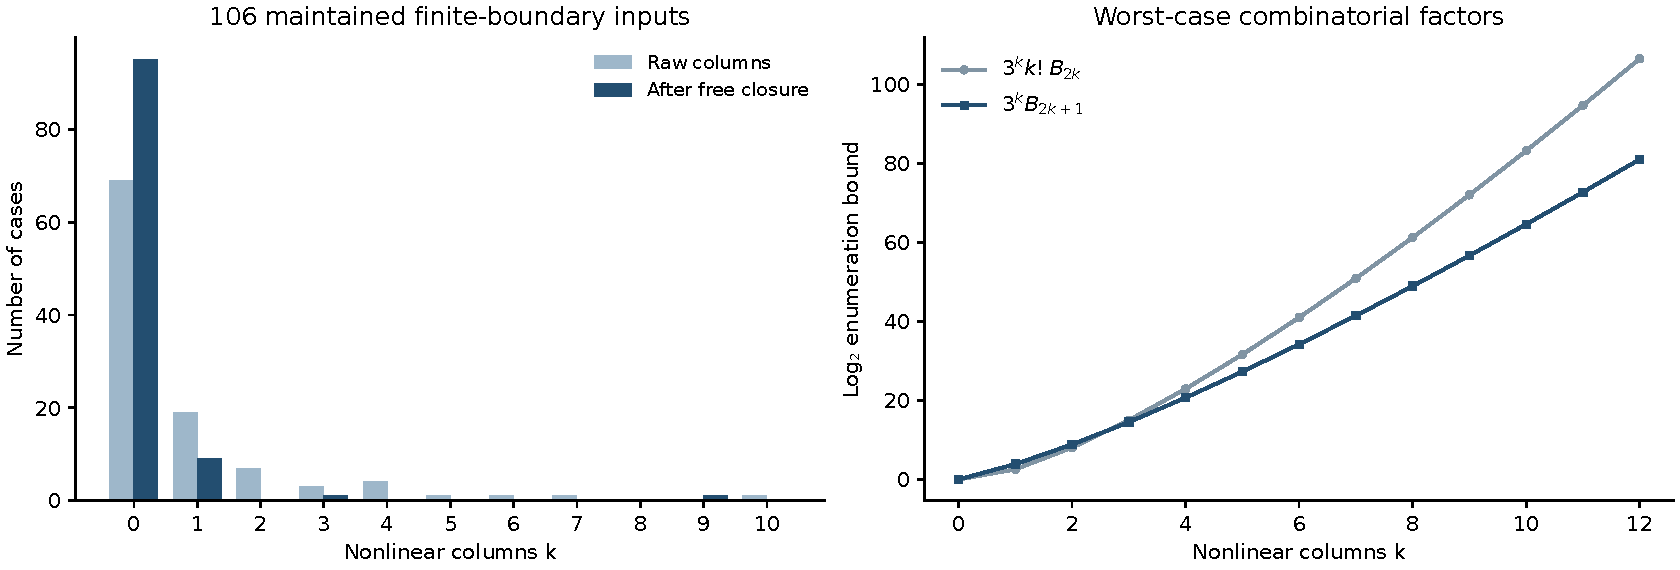
\includegraphics[width=\linewidth]{figures/parameters_and_bounds.pdf}
\caption{Left: measured raw and residual nonlinear parameters on the 106
maintained full-boundary inputs. Right: exact general enumeration factors
before data-dependent rank and closure pruning. The right panel depicts
combinatorial upper bounds, not measured running times.}
\label{fig:parameters}
\end{figure}

\subsection{Supplementary native stress cases and resource ceilings}

At a one-million structural-work allowance, the ordered strategy completes
228 of 234 questions: source $107/7/3$ and full boundary $99/15/3$, where
the entries denote success, no forest, and inconclusive. The output-only
strategy completes 232: source $109/7/1$ and full boundary $101/15/1$.
Every completed result is independently replayed and agrees with the
earlier exact reference. The only remaining output-only cap is the largest
stellar case, in both matrix variants.

The deterministic structural counters expose genuine improvements between
the two new strategies. On \texttt{stellar\_torus/3}, with residual $k=6$,
the count falls from 426,223 to 742. The output-only method completes
\texttt{stellar\_torus/4}, $k=9$, in 12,682 units, and
\texttt{nested\_interior\_torus/3}, $k=9$, in 397; the ordered strategy
reaches its cap on both. A unit of this instrumented work is not a machine
instruction or a portable elapsed-time unit. Counts from the older
implementation use different instrumentation and are not directly equated.

\subsection{Paired timings and ablations}

The paired benchmark uses all 117 native full-boundary matrices and 256
seeded relabelings described below, for 373 finite inputs. Each is run
seven times with a seeded random ordering of the six methods inside each
repetition. This yields 15,666 timed calls. Every complete timed answer
is independently checked outside the timer; there are 13,475 such
replays. Inconclusive results remain in the raw table.

The environment is CPython 3.12.14 on Linux. Geometry construction,
parameter reporting, and certificate replay are outside the timed region;
input parsing and search are inside it. The two new algorithms use the
same one-million work cap and are each run with rank pruning enabled and
disabled. The earlier stopping search uses its own 50,000-node cap;
these different counters do not represent equal computational budgets.
The machine-readable result retains every raw repetition, status, counter,
input hash, and code hash. Microsecond-scale timings characterize this run,
not a machine-independent performance promise.

\begin{center}
\begin{tabular}{@{}lrrrr@{}}
\toprule
Method & Success & No forest & Inconclusive & Median ($\mu$s) \\
\midrule
Earlier two-row solver & 67 & 2 & 37 & 42.80 \\
Earlier stopping search & 92 & 14 & 0 & 43.64 \\
Ordered events & 92 & 14 & 0 & 79.24 \\
Output assignments & 92 & 14 & 0 & 82.86 \\
\bottomrule
\end{tabular}
\end{center}


The output-only implementation has higher overhead than the existing
stopping search on most small instances. On the maintained corpus its
median per-input time is about 83 microseconds, compared with 44 for the
incumbent. Across the entire bank, it is faster on 16 of the 372 inputs
where both methods complete. The improvement in the parameterized
worst-case guarantee is therefore not a justification for replacing the
incumbent unconditionally.

\begin{center}
\begin{tabular}{@{}lrrrr@{}}
\toprule
Input & $k$ & Ordered (ms) & Output (ms) & Incumbent (ms) \\
\midrule
Stellar 1 & 0 & 0.068 & 0.080 & 0.058 \\
Stellar 2 & 3 & 0.111 & 0.129 & 0.143 \\
Stellar 3 & 6 & 309.743 & 0.614 & 0.296 \\
Stellar 4 & 9 & capped & 7.737 & 0.441 \\
Stellar 8 & 21 & capped & capped & 2.271 \\
Nested 1 & 1 & 0.135 & 0.139 & 0.165 \\
Nested 2 & 6 & 0.164 & 0.180 & 0.346 \\
Nested 3 & 9 & capped & 0.369 & 0.607 \\
\bottomrule
\end{tabular}
\end{center}


On the $k=6$ stellar case, the ordered median is 309.743 milliseconds
and the output-only median is 0.614 milliseconds, about a 505-fold
improvement. The incumbent still completes that input in 0.296
milliseconds. On the final nested case the output-only method takes
0.369 milliseconds, versus 0.607 for the incumbent, while the ordered
prototype is capped. Both favorable and unfavorable comparisons belong
in the integration decision.

The rank ablation is consequential on the harder stellar inputs. Removing
rank pruning changes the output-only $k=6$ median from 0.614 to 4.317
milliseconds, and makes its $k=9$ stellar run hit the work cap. It has
little or negative constant-factor effect on many tiny cases. The
largest stellar instance remains a useful counterweight to favorable
benchmarks: the incumbent finishes it in 2.271 milliseconds, while the
new output-only solver is still capped.

\subsection{Relabeling one source and evaluating the bounded prefix}

The 256 relabelings permute tetrahedra and local corners of the same
five-tetrahedron solid-torus zero cut, using seed 20261012471. The complete
finite tree oracle finds a successful tree in every instance. Native BFS
top selection succeeds on 238, and the existing native maximum-weight
choice succeeds on all 256. Both new exact solvers also succeed on all
256, with independently replayed saved certificates. These are labeled
variants of one manifold, not 256 new knot types. Since maximum weight
already covers the entire bank, the bank does not demonstrate additional
coverage from the new exact search.

The optional dispatcher in Section~\ref{sec:bounded-prefix} runs the
incumbent for at most $|R|+1$ search nodes before the FPT fallback. It
completes all 490 supplied source/full-boundary and relabeled questions,
with 468 successes and 22 exact negatives. Every answer is independently
checked. In this bank the incumbent always finishes within the prefix;
its maximum instrumented count is nine visited search nodes. Explicit separate controls exercise successful and negative
fallback certificates and the sparse huge-namespace route. These results
establish dispatcher correctness on the bank, not a measured speedup for
the wrapper or a universal nine-node bound.

\subsection{What can be reproduced without the repository}

The archive includes all finite input matrices, both runtime strategies,
their independent checkers, the pinned earlier finite comparator, saved
certificates, the full paired timing table, and a single reproduction
entry point. Those finite experiments require only the Python standard
library. Figure generation additionally uses Matplotlib; article building
uses a standard \LaTeX{} installation.

Reconstructing the native source geometry again requires the pinned
maintained runtime and the two named incoming geometry packages. The
included scripts accept explicit paths to them. Their file identities
and the source input vectors are retained, so this dependency is
reviewable and is not hidden behind the previously generated matrices.

\section{What the local theorem contributes to a quasi-polynomial bound}
\label{sec:global}

The useful improvement is a change of parameter. If the cap graph has
$s$ non-exterior vertices, straightforward top-tree search can have
depth $s$ and a branching factor depending on the matrix size. The present
algorithm permits arbitrary $s$ at each fixed number of nonlinear
columns. It gives a polynomial-time local operator for $k=0,1,2,\ldots$
held constant, with one uniform algorithm and a computable parameter factor.

Let $N_i$ be the encoded size of the $i$th supplied graph--matrix problem,
and let $k_i$ be its residual triple-column parameter. For a sequence of
$Q$ such calls, including unsuccessful calls, the local work is bounded by
\begin{equation}
 \sum_{i=1}^{Q}2^{O(k_i\log(k_i+2))}\operatorname{poly}(N_i).
 \label{eq:cumulative-local}
\end{equation}
The polynomial exponent is independent of $k_i$. If $N_i\le n^a$ and
$k_i\le K(n)$ for every call, this is at most
\[
             Q\,n^{O(1)}2^{O(K(n)\log(K(n)+2))}.
\]
Two parameter regimes make the scale concrete:
\begin{center}
\begin{tabular}{@{}ll@{}}
\toprule
Uniform residual parameter & Local cost for polynomial-size inputs \\
\midrule
$K(n)=O(\log n/\log\log n)$ & $n^{O(1)}$ \\
$K(n)=O(\log n)$ & $n^{O(\log\log n)}$ \\
$K(n)=O((\log n)^a)$, fixed $a>0$ &
$\exp(O((\log n)^a\log\log n))\,n^{O(1)}$ \\
\bottomrule
\end{tabular}
\end{center}
Under the additional uniform deficit hypothesis of
Corollary~\ref{cor:bounded-deficit}, bounded $\Delta$ sharpens the
$K(n)=O(\log n)$ line to polynomial local time. It also permits
$K(n)=O((\log n)^2)$ within $n^{O(\log n)}$ local time.

Small values of $n$ are absorbed into constants; the first line is an
asymptotic assertion as $n$ tends to infinity.

\begin{theorem}[Conditional transfer to an entire recognition procedure]
\label{thm:global-transfer}
Suppose an exact hierarchy procedure on an $n$-crossing input satisfies:
\begin{enumerate}
\item it makes at most $\exp(O((\log n)^b))$ calls to the present operator,
including calls made after resets and on failed branches;
\item each call has encoded size at most $n^a$ and residual nonlinear
premise budget at most $O((\log n)^c)$, for fixed $a,b,c$;
\item all other work, including surface discovery, source authentication,
marked geometric transport, and final certification, has a
quasi-polynomial total bound.
\end{enumerate}
Then substituting the present exact operator preserves a
quasi-polynomial total bound. More precisely, its contribution is
\[
 \exp\!\left(O((\log n)^b+(
                   \log n)^c\log\log n+\log n)\right).
\]
\end{theorem}
\begin{proof}
Apply the general premise-budget extension of
Theorem~\ref{thm:column-fpt} to every call, and use the uniform size and
parameter bounds in \eqref{eq:cumulative-local}. Multiplication by the
number of calls adds their logarithmic costs. The sum with the stated
quasi-polynomial bound for the other operations remains quasi-polynomial.
\end{proof}

This is an accounting theorem with explicit premises. The finite solver
proves none of the three hierarchy hypotheses by itself. In particular,
a polynomial encoded-time cut does not bound the number of candidate
surfaces or the number of restored hierarchy states. A small certificate
does not imply an efficient search for it.

The rank-layer reduction provides an additional structural direction.
Under native cycle compatibility, if a scenario leaves $p$ mandatory
source groups and $q$ residual demands, then it can succeed only if
$p\le r\le p+q$. The difference $r-p$ measures the number of
additional independent initial-seed witnesses needed to justify nonlinear
activation, beyond the mandatory unary source representatives. Controlling that difference, or decomposing the exceptional
columns into independently solvable regions, may be more feasible than
bounding every raw column count.

The current source experiments deliberately retain large-parameter cases.
Stellar subdivisions give examples with increasing numbers of nonlinear
columns while the underlying manifold remains a solid torus. This makes
clear why the same topological type, or small normal weight alone, cannot
justify assuming that every labelled raw instance has small $k$.

\section{Further research questions and proposed next steps}
\label{sec:future}

\begin{enumerate}[leftmargin=*,label=\textbf{\arabic*.}]
\item \textbf{Obtain single-exponential dependence on nonlinear columns.}
The distinguished-block theorem removes factorial event-order enumeration,
but unrestricted Bell partitions still give $2^{O(k\log k)}$. Bounded
rank deficit gives a single-exponential special case. Can representative
families, algebraic matroid methods, or a smaller exact state space reduce
this to $2^{O(k)}$? The required theorem must preserve shared predecessor
witnesses and external forest independence. Ordinary subset dynamic
programming that records only activated outputs can lose this information.

\item \textbf{Exploit the native rank layer before enumerating output assignments.}
The Stirling-layer theorem constrains the number of witness blocks. Can
the graphic rank and unary condensation force some output choices or
prerequisite support requirements in polynomial time? A certificate should make
each forced choice replayable and avoid assuming that a greedy surviving
row order is optimal.

\item \textbf{Use an interaction parameter.}
Several nonlinear columns may lie in disjoint regions of the unary
condensation. Can they be decomposed by separators or matroid sums while
retaining their shared forest constraint? The target is a cost exponential
in the largest interacting region, instead of the total number of
nonlinear columns.

\item \textbf{Choose the lower and upper forests together.}
The current theorem fixes the lower $0/1$ forest. Varying it changes the
matrix and its nonlinear parameter. Is there a source-relative operation
that reduces $k$ without creating a larger description or losing boundary
markings? The relevant goal is a certified joint optimization, not an
unverified algebraic simplification of attaching words.

\item \textbf{Implement weighted successful-forest optimization.}
The weighted theorem optimizes a linear cost over successful trees. A
production version could use retained raw passages or a proved upper
bound on later transport work as the objective. It should compare against
the existing unconstrained maximum-weight tree, and measure cases where
the latter leaves a stopping set.

\item \textbf{Recognize a certified matroidal activation regime.}
If the closure is itself a matroid closure, an additional intersection
gives a polynomial algorithm with no bound on $k$. Can native occurrence
data supply a compact certificate of that property? Chordal auxiliary
graphs give a concrete sufficient class; arbitrary circular Horn systems
do not satisfy the exchange axiom automatically.

\item \textbf{Transport the complete boundary pattern.}
The matrix certificate retains counts and source labels, while a hierarchy
also needs cyclic order, orientations, and marked peripheral data.
Construct a compiler that turns every selected tree and peel trace into
the required marked homeomorphism with a bound on the accumulated encoding.
The currently authenticated port charts are a starting point.

\item \textbf{Extend the available cancellation moves.}
A complete negative forest certificate isolates a genuine limitation of
the fixed raw model. Investigate source-authenticated handle slides,
disk-bundle absorption, or controlled retriangulations on those residuals.
The progress measure should charge the representation growth as well as
the reduction in the number of handles.

\item \textbf{Develop smaller negative certificates.}
Exhaustive scenario/partition coverage is fixed-parameter sized but can
be much larger than a positive trace. Can several Rado deficiencies share
one succinct implication or rank certificate? A proposed compression must
prove that every omitted scenario is covered, rather than merely retain
a log of explored branches.

\item \textbf{Prove geometric bounds on the residual parameter.}
Does a well-chosen admissible hierarchy admit $k=O(\log n)$, or a
polylogarithmic total nonlinear premise budget after each free closure?
Counterexamples should distinguish poor labelled triangulations from an
unavoidable obstruction across all allowed normalizations.

\item \textbf{Account for the entire search history.}
Combine the local primitive with constructive versions of surface
discovery, hierarchy repair, and the quantitative multi-surface steps in
the announced algorithm. A complete bound must include failed branches,
restarts, certificate replay, and all input bits created along the way.

\item \textbf{Formalize the finite core first.}
The closure, scenario, separated-demand, and partition lemmas have finite
combinatorial statements and modest dependencies. They are suitable first
targets for Lean formalization. The geometric interpretation should be
formalized separately, so that verification of the finite search is not
mistaken for a formal proof of the manifold compiler.
\end{enumerate}

% Suggested bibliography fragment for the article.  Requires hyperref or url.
% Bibliographic identities checked against primary publisher/author sources.
% The three repository items are incoming research drafts, not publications.
\begingroup
\raggedright
\begin{thebibliography}{99}

\bibitem{repo-positive}
ProveIt research continuation,
\emph{Rectangular Cancellation Without Search:
Stopping-set certificates, exact passive transport, and deferred-handle
kernels for unknot recognition}, 12 October 2026.
Incoming research package
\texttt{ProveIt\_Positive\_Cancellation\_2026-10-12.zip}.
\url{https://github.com/VladimirReshetnikov/ProveIt/tree/ada929648530f8689c26426e132a1b3e1c69c724/docs/incoming}.

\bibitem{repo-dual-normalization}
ProveIt research continuation,
\emph{Dual Forest Normalization and Constrained Cancellation for
Compressed Unknot Hierarchies}, 12 October 2026.
Incoming research package
\texttt{ProveIt\_Dual\_Forest\_Normalization\_2026-10-12.zip}.
\url{https://github.com/VladimirReshetnikov/ProveIt/tree/ada929648530f8689c26426e132a1b3e1c69c724/docs/incoming}.

\bibitem{repo-relative-top}
ProveIt research continuation,
\emph{Relative Top-Handle Elimination and the Limits of Forest
Optimization in Compressed Unknot Recognition}, 12 October 2026.
Incoming research package
\texttt{ProveIt\_Relative\_Top\_Handles\_2026-10-12.zip}.
\url{https://github.com/VladimirReshetnikov/ProveIt/tree/ada929648530f8689c26426e132a1b3e1c69c724/docs/incoming}.

\bibitem{lackenby-davis}
Marc Lackenby,
\emph{Unknot recognition in quasi-polynomial time},
Davis lecture slides, February 2021.
\url{https://people.maths.ox.ac.uk/lackenby/quasipolynomial-talk.pdf}.

\bibitem{lackenby-oxford}
Marc Lackenby,
\emph{Unknot recognition in quasi-polynomial time},
Oxford lecture slides, March 2021.
\url{https://people.maths.ox.ac.uk/lackenby/quasipolynomial-talk-oxford.pdf}.

\bibitem{lackenby2026}
Marc Lackenby,
\emph{Incompressible surfaces, hierarchies and unknot recognition},
arXiv:2607.23350v1, 25 July 2026.
\url{https://arxiv.org/abs/2607.23350v1}.

\bibitem{horn-keys}
Krist\'of B\'erczi, Endre Boros, Ond\v{r}ej \v{C}epek,
Petr Ku\v{c}era, and Kazuhisa Makino,
\emph{Unique key Horn functions},
Theoretical Computer Science \textbf{922} (2022), 170--178.
\url{https://doi.org/10.1016/j.tcs.2022.04.022}.

\bibitem{hypergraph-horn}
Krist\'of B\'erczi, Endre Boros, and Kazuhisa Makino,
\emph{Hypergraph Horn Functions},
SIAM Journal on Discrete Mathematics \textbf{38}(2) (2024), 1417--1437.
\url{https://doi.org/10.1137/23M1569162}.
Author preprint: \url{https://arxiv.org/abs/2301.05461}.

\bibitem{stopping-sets}
Anxiao Jiang et al.,
\emph{Stopping Set Elimination for LDPC Codes},
2017 55th Annual Allerton Conference on Communication, Control,
and Computing (2017), 700--707.
\url{https://doi.org/10.1109/ALLERTON.2017.8262806}.
Author manuscript:
\url{https://people.engr.tamu.edu/ajiang/Publications/2017/StoppingSetElimination_Allerton.pdf}.

\bibitem{uniquely-restricted}
Martin Charles Golumbic, Tirza Hirst, and Moshe Lewenstein,
\emph{Uniquely Restricted Matchings},
Algorithmica \textbf{31} (2001), 139--154.
\url{https://doi.org/10.1007/s00453-001-0004-z}.

\bibitem{rado}
Richard Rado,
\emph{A theorem on independence relations},
The Quarterly Journal of Mathematics \textbf{os-13}(1) (1942), 83--89.
\url{https://doi.org/10.1093/qmath/os-13.1.83}.

\bibitem{edmonds}
Jack Edmonds,
\emph{Matroid intersection},
in P.~L.~Hammer, E.~L.~Johnson, and B.~H.~Korte (eds.),
\emph{Discrete Optimization I},
Annals of Discrete Mathematics \textbf{4} (1979), 39--49.
\url{https://doi.org/10.1016/S0167-5060(08)70817-3}.

% Optional entries for the alternative matroidal-closure regime or a fuller
% discussion of triangular certificates; remove if unused in the article.
\bibitem{matroid-horn}
Krist\'of B\'erczi, Endre Boros, and Kazuhisa Makino,
\emph{Matroid Horn functions},
Journal of Combinatorial Theory, Series A \textbf{203} (2024), 105838.
\url{https://doi.org/10.1016/j.jcta.2023.105838}.
Author preprint: \url{https://arxiv.org/abs/2301.06642}.

\bibitem{zero-forcing}
Maguy Tr\'efois and Jean-Charles Delvenne,
\emph{Zero forcing number, constrained matchings and strong structural
controllability},
Linear Algebra and its Applications \textbf{484} (2015), 199--218.
\url{https://doi.org/10.1016/j.laa.2015.06.025}.

\end{thebibliography}
\endgroup

\end{document}
